\documentclass[tikz,border=10pt]{standalone}
% No extra TikZ libraries are needed for this figure.
\begin{document}
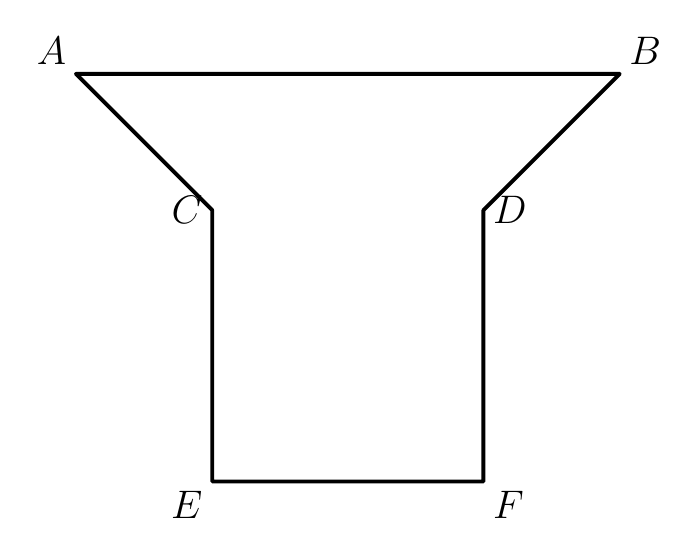
\begin{tikzpicture}[line join=round]
  % Vertices: pixel -> cm, s = 0.018223, centre (256.5,187.5), y flipped
  \coordinate (A) at (-3.453,  2.597);
  \coordinate (B) at ( 3.453,  2.597);
  \coordinate (C) at (-1.722,  0.866);
  \coordinate (D) at ( 1.722,  0.866);
  \coordinate (E) at (-1.722, -2.579);
  \coordinate (F) at ( 1.722, -2.579);

  % Closed polygon A-B-D-F-E-C, solid black, no fill
  \draw[line width=1.4pt, color=black] (A) -- (B) -- (D) -- (F) -- (E) -- (C) -- cycle;

  % Vertex labels placed outside the polygon
  \node[above left,  font=\fontsize{14.5}{17.4}\selectfont] at (A) {$A$};
  \node[above right, font=\fontsize{14.5}{17.4}\selectfont] at (B) {$B$};
  \node[left,        font=\fontsize{14.5}{17.4}\selectfont] at (C) {$C$};
  \node[right,       font=\fontsize{14.5}{17.4}\selectfont] at (D) {$D$};
  \node[below left,  font=\fontsize{14.5}{17.4}\selectfont] at (E) {$E$};
  \node[below right, font=\fontsize{14.5}{17.4}\selectfont] at (F) {$F$};
\end{tikzpicture}
\end{document}